% !TeX root = ../main.tex
\section{Material form of conservation of mass}
%
\begin{figure}
	\centering
	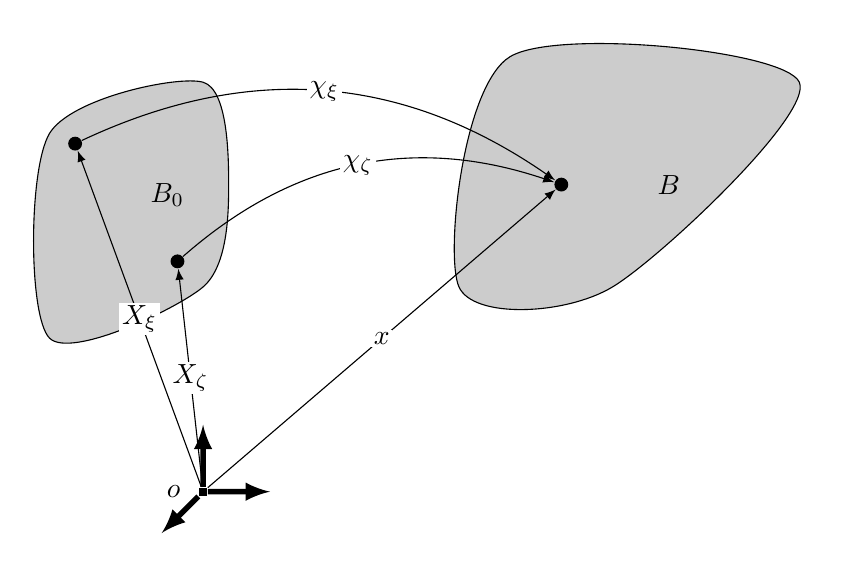
\begin{tikzpicture}[scale=0.65]
		\tikzstyle{pt}=[circle, fill=black, inner sep=0pt, minimum size=5pt]
		\draw [black, fill=black!20] plot [smooth cycle] coordinates {(-1.0,-1.0) (2,0) (2.5,2) (2,4) (-1,3)};
		\draw [black, fill=black!20] plot [smooth cycle] coordinates {(7, 0) (10,0) (13.65, 4) (8,4.5)};
		\draw (2,-4) node[fill=black, minimum size=3pt, inner sep=0pt, label={[label distance=3pt]180:$o$}] (O) {} ;
		\draw (-0.5,2.8) node[pt] (Xf) {} ;
		\draw (1.5,0.5) node[pt] (Xs) {} ;
		\draw (9.0,2) node[pt] (x) {} ;
		\draw[-latex] (O) -- (Xf) node[midway, fill=white, inner sep=1pt] {$\mbf{X}_\xi$} ;
		\draw[-latex] (O) -- (Xs) node[midway, fill=white, inner sep=1pt] {$\mbf{X}_\zeta$} ;
		\draw[-latex] (O) -- (x) node[midway, fill=white, inner sep=1pt] {$\mbf{x}$} ;
		\draw[bend left, -latex] (Xs) to node[midway, fill=white, inner sep=1pt] {$\bs{\chi}_\zeta$} (x);
		\draw[bend left, -latex] (Xf) to node[midway, fill=white, inner sep=1pt] {$\bs{\chi}_\xi$} (x);
		\draw (1.3,1.8) node () {${\mc{B}_0}$} ;
		\draw (11.1,2) node () {${\mc{B}}$} ;
		\draw (3.5,-4) node (xaxis) {} ;
		\draw (2,-2.5) node (yaxis) {} ;
		\draw (1.0,-5.0) node (zaxis) {} ;
		\draw[-latex, line width=2pt] (O) -- (xaxis)  {} ;
		\draw[-latex, line width=2pt] (O) -- (yaxis)  {} ;
		\draw[-latex, line width=2pt] (O) -- (zaxis)  {} ;
	\end{tikzpicture}
	\caption{Schematic description of mixture kinematics showing the deformation maps, $\bs\chi_\xi$, linking phase reference configurations, $\mbf{X}_\xi$, to the common current configuration, $\mbf{x}$.}
	\label{fig:component_kinematics}
\end{figure}
%
We consider a mixture whose phases occupy a common current configuration
$\mc B$.  The phase label $\xi$ identifies all material that moves with the same
motion $\bs\chi_\xi$, while the component label $\alpha$ distinguishes chemical
species or constituents within that phase.  This convention permits fluids,
gases, and solids to be treated with one notation: a phase is the collection of
components that share the trajectory $\bs\chi_\xi$.  Given a differential mass
${\rm d}m^\al_\xi$ of component $\al$ in phase $\xi$, define the component
partial density per current mixture volume by
%
% AGENT-LOCK-BEGIN equation-lock: do not edit unless explicitly unlocked by user
\begin{equation}
	\rho^\al_\xi(\mbf{x}, t) = \frac{{\rm d}m^\al_\xi}{\dv},
	\label{eq:component_partial_density_definition}
\end{equation}
% AGENT-LOCK-END
%
where $\dv = {\rm d}x_1 {\rm d}x_2 {\rm d}x_3$ is a current-configuration volume
element of the mixture.  Each phase is tracked from its own reference
coordinates $\mbf X_\xi$ and reference volume element
%
% AGENT-LOCK-BEGIN equation-lock: do not edit unless explicitly unlocked by user
\begin{equation}
	\dVxi = ({\rm d}X_1)_\xi({\rm d}X_2)_\xi({\rm d}X_3)_\xi.
	\label{eq:phase_reference_volume_element}
\end{equation}
% AGENT-LOCK-END
%
The phase reference coordinates are related to the common current coordinates by
a one-to-one, invertible, and continuously differentiable map on the region where
that phase is present,
%
% AGENT-LOCK-BEGIN equation-lock: do not edit unless explicitly unlocked by user
\begin{equation}
	\mbf{x} = \bs{\chi}_\xi(\mbf{X}_\xi,t),
	\label{eq:phase_motion_map}
\end{equation}
% AGENT-LOCK-END
%
with phase deformation gradient $\mbf{F}_\xi$ and Jacobian
%
% AGENT-LOCK-BEGIN equation-lock: do not edit unless explicitly unlocked by user
\begin{align}
	J_\xi & = \det\left(\p{\bs{\chi}_\xi}{\mbf{X}_\xi}\right), \notag \\
	      & = \det\left(\mbf{F}_\xi\right).
	\label{eq:phase_jacobian_definition}
\end{align}
% AGENT-LOCK-END
%
Let $\rho_{\xi0}^\al(\mbf X_\xi)$ denote the initial component partial density,
evaluated at $\mbf x(t=0)=\mbf X_\xi$.  Let
$\mathcal{C}^\al_\xi(\mbf X_\xi,t)$ denote the mass of component $\alpha$ added
to phase $\xi$ per unit phase reference volume by internal conversion.  Internal
conversion includes chemical reactions and pure phase transformations.  The
component mass balance in integral form is
%
% AGENT-LOCK-BEGIN equation-lock: do not edit unless explicitly unlocked by user
\begin{align}
	\int_{\mc{B}_{\xi 0}} \left(\rho_{\xi 0}^\al + \mc{C}^\al_\xi\right)\dVxi
	 & = \int_{\mc{B}} \rho_\xi^\al \dv                     \\
	 & = \int_{\mc{B}_{\xi 0}} \rho_{\xi}^\al J_\xi \dVxi .
	\label{eq:material_mass}
\end{align}
% AGENT-LOCK-END
%
where the last equality pulls the current integral back to the phase reference
configuration $\mc B_{\xi0}$.  The Jacobian $J_\xi$ accounts for the change in
volume between the phase reference configuration and the common current
configuration.
%

Since \eqref{eq:material_mass} must hold for arbitrary $\mc{B}_{\xi0}$,
%
% AGENT-LOCK-BEGIN equation-lock: do not edit unless explicitly unlocked by user
\begin{equation}
	\rho_{\xi 0}^\alpha + \mc{C}^\alpha_\xi = \rho_\xi^\alpha J_\xi.
	\label{eq:material_mass_2}
\end{equation}
% AGENT-LOCK-END
%
The material time derivative of a quantity $\square_\xi$ observed along the
velocity of phase $\zeta$ is
%
% AGENT-LOCK-BEGIN equation-lock: do not edit unless explicitly unlocked by user
\begin{equation}
	\frac{D_\zeta \square_\xi}{Dt}
	= \frac{\partial \square_\xi}{\partial t}
	+ \mbf{v}_\zeta \cdot\nabla_{\mbf{x}}\square_\xi,
	\label{eq:phase_material_time_derivative_definition}
\end{equation}
% AGENT-LOCK-END
%
where $\nabla_{\mbf x}$ is the spatial gradient operator.  We use the shorthand
$\dot\square_\xi = D_\xi \square_\xi/Dt$ for the material time derivative
following phase $\xi$.  Taking the material time derivative of
\eqref{eq:material_mass_2} following phase $\xi$ and using the identity
$\dot J_\xi = J_\xi \nabla_{\mbf x}\cdot\mbf v_\xi$ gives
%
% AGENT-LOCK-BEGIN equation-lock: do not edit unless explicitly unlocked by user
\begin{align}
	\frac{D_\xi \rho_\xi^\alpha}{Dt}
	+ \rho_\xi^\alpha \nabla_\mbf{x}\cdot\mbf{v}_\xi
	 & = \frac{\dot{\mc {C}}^\alpha_\xi}{J_\xi} .
	\label{eq:component_material_mass}
\end{align}
% AGENT-LOCK-END
%
We define the current production rate per unit current mixture volume by
%
% AGENT-LOCK-BEGIN equation-lock: do not edit unless explicitly unlocked by user
\begin{equation}
	\dot{c}^\al_\xi(\mbf{x},t) \equiv \frac{\dot{\mc{C}}^\al_\xi}{J_\xi}.
	\label{eq:current_conversion_rate_definition}
\end{equation}
% AGENT-LOCK-END
%
Expanding \eqref{eq:component_material_mass} gives the spatial component mass
balance for phase $\xi$:
%
% AGENT-LOCK-BEGIN equation-lock: do not edit unless explicitly unlocked by user
\begin{align}
	\frac{\partial \rho_\xi^\alpha}{\partial t}
	+ \nabla_\mbf{x}\cdot\left(\rho_\xi^\alpha\mbf{v}_\xi\right)
	= \dot{c}^\alpha_\xi .
	\label{eq:component_spatial_mass}
\end{align}
% AGENT-LOCK-END
%
Introduce the phase partial density
$\rho_\xi = \sum_\alpha \rho_\xi^\alpha$ and the mass fraction of component
$\alpha$ in phase $\xi$,
%
% AGENT-LOCK-BEGIN equation-lock: do not edit unless explicitly unlocked by user
\begin{equation}
	\eta^\alpha_\xi = \frac{\rho^\alpha_\xi}{\rho_\xi},
	\label{eq:phase_mass_fraction}
\end{equation}
% AGENT-LOCK-END
%
Summing \eqref{eq:phase_mass_fraction} over $\al$ gives the mass-fraction
constraint within phase $\xi$:
%
% AGENT-LOCK-BEGIN equation-lock: do not edit unless explicitly unlocked by user
\begin{equation}
	\sum_\alpha \eta_\xi^\alpha = 1.
	\label{eq:mass_fraction_constraint}
\end{equation}
% AGENT-LOCK-END
The phase volume fraction is defined as
% AGENT-LOCK-BEGIN equation-lock: do not edit unless explicitly unlocked by user
\begin{equation}
	\phi_\xi = \frac{\dv_\xi}{\dv},
	\label{eq:phase_volume_fraction}
\end{equation}
% AGENT-LOCK-END
and summing over $\xi$ gives the volume-fraction constraint:
% AGENT-LOCK-BEGIN equation-lock: do not edit unless explicitly unlocked by user
\begin{equation}
	\sum_\xi \phi_\xi  = 1.
	\label{eq:volume_fraction_constraint}
\end{equation}
% AGENT-LOCK-END
%
The phase intrinsic density is
$\bar\rho_\xi = {\rm d}m_\xi/\dv_\xi$, so that
%
% AGENT-LOCK-BEGIN equation-lock: do not edit unless explicitly unlocked by user
\begin{subequations}
	\begin{align}
		\rho_\xi        & = \phi_\xi \bar\rho_\xi,
		\label{eq:phase_partial_density_representation}            \\
		\rho_\xi^\alpha & = \phi_\xi \bar\rho_\xi \eta^\alpha_\xi.
		\label{eq:component_partial_density_representation}
	\end{align}
\end{subequations}
% AGENT-LOCK-END
%
Substituting \eqref{eq:component_partial_density_representation} into
\eqref{eq:component_spatial_mass} and summing over phases gives the global
component mass balance:
%
% AGENT-LOCK-BEGIN equation-lock: do not edit unless explicitly unlocked by user
\begin{align}
	\frac{\partial}{\partial t}\left(\sum_\xi \phi_\xi \bar\rho_\xi \eta^\al_\xi\right)
	+ \nabla_\mbf{x}\cdot\left( \sum_\xi \phi_\xi \bar\rho_\xi \eta^\al_\xi \mbf{v}_\xi\right)
	= \sum_\xi \dot{c}^\alpha_\xi .
	\label{eq:spatial_mass_2}
\end{align}
% AGENT-LOCK-END
%
Internal conversion is represented by current progress rates $\dot r_{(m)}$
together with phase/component stoichiometric coefficients
$\nu_{\xi (m)}^\alpha$.  The current production rate is
%
% AGENT-LOCK-BEGIN equation-lock: do not edit unless explicitly unlocked by user
\begin{equation}
	\dot{c}_\xi^\alpha = \sum_m \nu_{\xi(m)}^\alpha \dot{r}_{(m)} .
	\label{eq:unified_stoich_current}
\end{equation}
% AGENT-LOCK-END
%
The mechanism index $(m)$ includes chemical reactions and pure phase
transformations.  A pure phase transformation of component $\alpha$ from phase
$\xi$ to phase $\zeta$ is the special one-to-one stoichiometry
$\nu_{\xi (m)}^\alpha=-1$, $\nu_{\zeta (m)}^\alpha=+1$, with all other entries
zero.  A chemical reaction may change both component identity and phase label.
Substituting \eqref{eq:unified_stoich_current} into \eqref{eq:spatial_mass_2}
and summing over $\al$ gives the overall mass balance
% AGENT-LOCK-BEGIN equation-lock: do not edit unless explicitly unlocked by user
\begin{align}
	\frac{\partial}{\partial t}\left(\sum_\xi \sum_\al \phi_\xi \bar\rho_\xi \eta^\al_\xi\right)
	+ \nabla_\mbf{x}\cdot\left( \sum_\xi \sum_\al \phi_\xi \bar\rho_\xi \eta^\al_\xi \mbf{v}_\xi\right)
	 & = \sum_\xi \sum_\al \nu^\alpha_{\xi (m)} \dot{r}_{(m)},
	\label{eq:spatial_mass_3}
\end{align}
% AGENT-LOCK-END
or equivalently,
% AGENT-LOCK-BEGIN equation-lock: do not edit unless explicitly unlocked by user
\begin{align}
	\dot{\rho} + \nabla_\mbf{x} \cdot \left( \rho \mbf{v} \right) & = 0.
	\label{eq:spatial_mass_4}
\end{align}
% AGENT-LOCK-END
where $\rho = \sum_\xi \rho_\xi$ is the mixture density and $\mbf v$ is the
barycentric mixture velocity
% AGENT-LOCK-BEGIN equation-lock: do not edit unless explicitly unlocked by user
\begin{align}
	\mbf{v} = \frac{1}{\rho} \sum_\xi \rho_\xi \mbf{v}_\xi
\end{align}
% AGENT-LOCK-END
%
The right-hand side of \eqref{eq:spatial_mass_3} vanishes by stoichiometric mass
conservation for each internal mechanism:
$\sum_\xi\sum_\alpha\nu_{\xi (m)}^\alpha=0$.

The variational derivation below treats $\mathcal C_\xi^\alpha$, $J_\xi$, and
the mechanism rates $\dot r_{(m)}$ as primitive quantities.  The current
production rate $\dot c_\xi^\alpha$ is therefore not independent; it is the
current-volume representation of the reference production rate.  This produces
the conversion constraint
% AGENT-LOCK-BEGIN equation-lock: do not edit unless explicitly unlocked by user
\begin{align}
	\sum_\al \sum_\xi \left(\frac{\dot{\mc{C}^\al_\xi}}{J_\xi} -  \sum_m \nu^\al_{\xi (m)} \dot{r}_{(m)} \right) = 0.
\end{align}
% AGENT-LOCK-END
